\section{導入}

\subsection{計算可能解析}

計算可能解析 (Computable Analysis) では計算可能性理論や計算量理論の視点から解析学を扱う. 
「計算可能な実数」や「多項式時間計算可能な実関数」といった概念を定義し, 
解析学に現れる様々な実数や実関数の本質的な難しさを分析する. 

離散的な対象においては「計算できる関数」はモデルによらず,
すべてチューリング機械で計算できるものと同値であることが知られているが,
実数計算においては, 計算できる関数が互いに異なる, いくつかのモデルが提唱されている.
本稿では,
「機械が実関数を計算する」ことを次のように定義する.

実関数 $f \colon \R \to \R$ を計算するといっても,
実数は有限の文字列で表されないため,
機械がその完全な値を読み書きすることはできない.
そこで実数を近似値の列で表現する.
有理数の列 $(r_n)_n$ が $x$ を表現するとは,
$(r_n)_n$ が $x$ へ速く収束すること, 
すなわち $|r_n - x| \le 2^{-n}$ を満たすこととする.
数列は $n \in \N$ を $r_n \in \Q$ へ移す関数と考えることもでき,
そのような関数または数列を実数の名と呼ぶ.

実関数を計算するモデルとしては神託チューリング機械を用いる. 
ある機械が関数 $f \colon [0, 1] \to \R$ を計算するとは,
入力となる実数 $x$ の名を神託として与えられ,
求める精度 $n$ を入力として与えられたとき,
有理数 $s_n$ で $|s_n - f(x)| \le 2^{-n}$ を満たすものを出力することとする.

この神託機械の資源を制限することで, 
実関数が多項式時間計算可能, 或いは多項式領域計算可能であることを
定義できる (\ref{section: preliminaries}節).

\subsection{問題と関連研究}

連続実関数 $g \colon [0,1] \times \R \to \R$ にたいして次の常微分方程式を考える. 
\begin{align}
 \label{eq:ode}
 h(0) & = 0, &
 h'(t) & = g(t,h(t)) \quad (t \in [0,1])
\end{align}
本稿では $g$ が多項式時間計算可能であるとき, 
解 $h$ がどれほど複雑でありうるかを考える.

$g$ に他に何の制限も設けない場合, 解 $h$ (一般に一意でない) は計算不能たりうるため,
様々な制限のもと $h$ の計算量が研究されている (表 \ref{table:related}).
この表では下に向うにつれて左列の条件が強まっている. 
Lipschitz 条件とは解 $h$ が一意であるための十分条件であり, 
これが満たされるときには, 解 $h$ は多項式領域計算可能であり, 
$\PSPACE$ 困難 (\ref{section: preliminaries}節で定義) でありうることがわかっている. 
つまり上界と下界が一致しているといえる (詳しくは河村 \cite{kawamura2010lipschitz}).
一方で $g$ が解析的であるとき, 解 $h$ も解析的となり, 
このとき $h$ は多項式時間計算可能である.

\begin{table}
\renewcommand\arraystretch{1.5}
\begin{center}
 \caption{多項式時間計算可能関数 $g$ の常微分方程式 (\ref{eq:ode}) の解 $h$ の計算量}
 \label{table:related}
 \begin{tabular}{lll}
  制限 & 上界 & 下界 \\
  \hline
   --- & --- & 計算不可能たりうる \cite{pour1979computable} \\
  $h$ が $g$ の唯一解 & 計算可能 \cite{coddington1955theory}
  & 任意の時間がかかりうる \cite{ko1983computational} \cite{miller1970recursive} \\
  $g$ が Lipschitz 条件を満たす & 多項式領域計算可能
      &	\PSPACE 困難になりうる \cite{kawamura2010lipschitz}\\
  $g$ が $(0, 1)$ 回連続微分可能 & 多項式領域計算可能 & \parbox[t]{14zw}{\PSPACE 困難になりうる\\{}[本稿定理\ref{DifferentiableIsPspace}]} \\
  $g$ が $(0, k)$ 回連続微分可能 & 多項式領域計算可能 & \parbox[t]{14zw}{\DIVPlog 困難たりうる\\{}[本稿定理\ref{KTimesIsPspace}]} \\
  $g$ が解析的 
  & 多項式時間計算可能 \cite{ko1988computing} \cite{kawamura2010complexity} 
  & ---
 \end{tabular}
\end{center}
\end{table}

そこで本稿ではこの隔たりを埋めるため, 滑らかな関数, 
つまり微分可能な $g$ について $h$ の計算量がどれほどになりうるかを調べ,
以下の結果を得た.

 \begin{theorem}
  \label{DifferentiableIsPspace}
  多項式時間計算可能かつ $(\infty, 1)$ 回連続的微分可能な
  実関数 $g \colon [0,1] \times [-1,1] \to \R$ であって, 
  常微分方程式(\ref{eq:ode})が
  $\PSPACE$ 困難な解 $h \colon [0, 1] \to \R$ をもつものが存在する.
 \end{theorem}

 \begin{theorem}
  \label{KTimesIsPspace}
  任意の自然数 $k \ge 2$ にたいして, 
  多項式時間計算可能かつ $(\infty, k)$ 回連続的微分可能な
  実関数 $g \colon [0,1] \times [-1,1] \to \R$ であって, 
  常微分方程式(\ref{eq:ode})が
  $\DIVPlog$ 困難な解 $h \colon [0, 1] \to \R$ をもつものが存在する.
 \end{theorem}

ここで $g \colon [0,1] \times \R \to \R$ でなく
$g \colon [0,1] \times [-1, 1] \to \R$ と書いたのは, 
本稿では実関数の多項式時間計算可能性を, 
定義域が有界閉領域のときにのみ定義するからである. 
このため $h$ が区間 $[-1, 1]$ の外に値を取ることがあると
方程式(\ref{eq:ode})が意味をなさなくなるが, 
定理\ref{DifferentiableIsPspace}, \ref{KTimesIsPspace}において $h$ が
解であるというのは, 
任意の $t \in [0, 1]$ について $h (t) \in [-1, 1]$ が満たされることも含めて述べている.
なお両定理とも Lipschitz 条件よりも強い仮定を置いているため, 
そのような $h$ は $g$ に対して, 存在すれば唯一である. 

 $\DIVPlog$ とは本稿において定義される計算量クラスであり,
 $\DIVPlog \subseteq \PSPACE$ であるが, $\DIVPlog = \PSPACE$ か否かは未解決であるため,
 $(\infty, k)$回連続微分可能関数の常微分方程式の解が \PSPACE 困難になりうるかは
 わからない.
 厳密な定義は次節で導入する.

 二変数関数 $g$ が $(i, j)$ 階連続微分可能であるとは,
 第一変数について $i$ 回, 第二変数について $j$ 回微分可能であり,
 その導関数が連続であることと定義する.
 この定義は一般的な多変数関数における $k$ 階連続的微分可能の定義
 (任意の $k$ 階導関数が存在し, それらがすべて連続)とは異なる.
 $(i,j)$ 回連続微分可能であれば $\min \{i, j\}$ 回連続微分可能であるため,
 定理 \ref{DifferentiableIsPspace}, \ref{KTimesIsPspace} は
 それぞれ $1$ 回連続微分可能, $k$ 回連続微分可能と置き換えても成り立つ.

 また定理 \ref{KTimesIsPspace} において
 任意の $k$ に対して $(\infty, k)$ 階微分可能な関数を考えているが,
 一つの関数が任意の $k$ にたいして $k$ 階微分であることを求めているわけではない.
 つまり $g$ が無限回微分可能であると制限しているわけではない. 
 無限回微分可能な関数に対する常微分方程式の計算量は今後の課題である.





\subsection{差分方程式}
\label{section:divp}

定理 \ref{DifferentiableIsPspace} と定理 \ref{KTimesIsPspace} の証明の中では,
まず滑らかな実関数の常微分方程式で模倣できる離散版常微分方程式を考え, 
その「離散版常微分方程式」がある計算量クラスについて困難であることを示している.
この節ではその離散版常微分方程式である, 
差分方程式と差分方程式に対応する計算量クラスについて定義する.



$[n] = \{0, \dots , n-1\}$ と表記する.
関数 $G \colon [P] \times [Q] \times [R] \to \{-1, 0, 1\}$ にたいして,
関数 $H \colon [P + 1] \times [Q+1] \to [R]$ が
任意の $i \in [P],\ T \in [Q]$ について以下を満たすとき,
$H$ を $G$ の差分方程式の解と呼ぶ.
\begin{gather}
   H(i, 0) = H(0, T) = 0 
\\
   H(i + 1, T + 1) = H(i+1, T) + G(i, T, H(i, T))  \label{eq:divp}
\end{gather}
$P, Q, R$ のことをそれぞれ行数, 列数, 欄の大きさと呼ぶ.
$G$ と $H$ が常微分方程式の $g$ と $h$ に対応し,
$H(i, 0) = 0$ と言う条件が $h(0) = 0$,
式 (\ref{eq:divp}) と同値である $H(i + 1, T + 1) - H(i+1, T) = G(i, T, H(i, T))$
と言う条件が $h'(t) = g(t, h(t))$ と対応する.

 言語 $L$ にたいして, 
 \begin{equation}
	L(u) = \begin{cases} 
	       1 & u \in L \\
	       0 & u \not \in L 
	       \end{cases}
 \end{equation}
 と表記する.
 言語 $L$ が $(G_u)_u$ の差分方程式によって認識されるとは,
 各 $u$ にたいして $G_u$ の段数と列数, 解をそれぞれ $P_u, Q_u, H_u$ としたとき,
 $H_u(P_u, Q_u) = L(u)$ をみたすこととする[表 \ref{fig:divp}].



 \begin{figure}
  \label{fig:divp}
  \begin{center}
   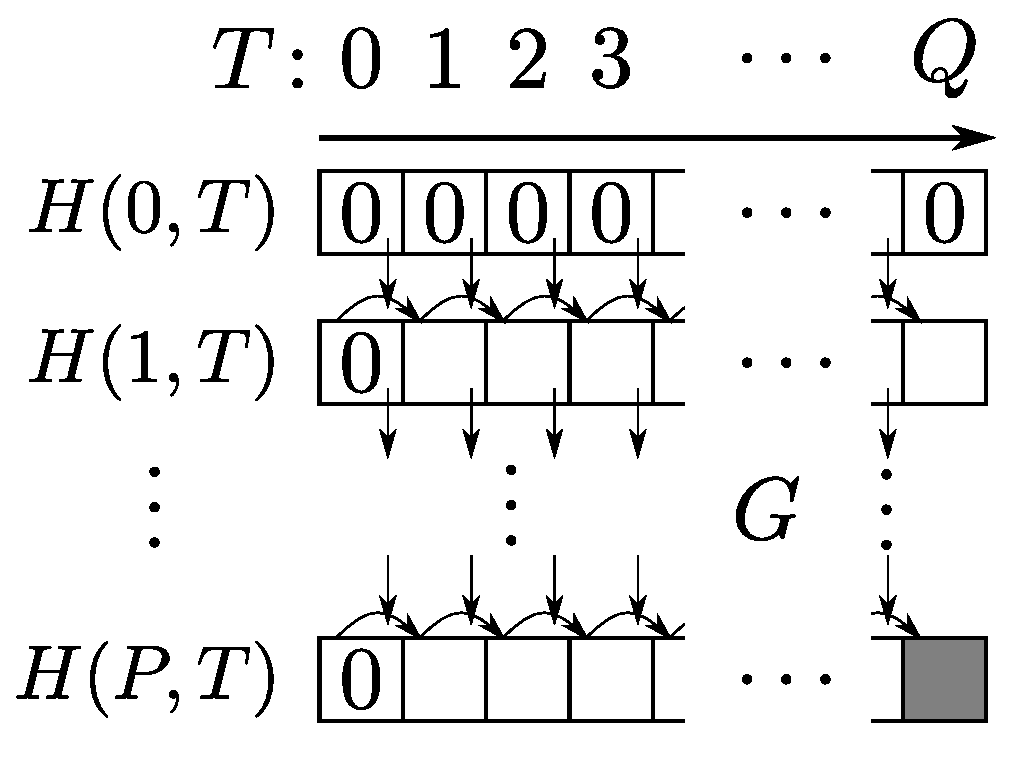
\includegraphics[height=0.2\textheight]{image/divp.eps}
  \end{center}
  \caption{差分方程式}
 \end{figure}



 段数が $|u|$ の多項式で抑えられ, $G_u$ が多項式時間計算可能な
 差分方程式について考えたい.
 $(G_u)_u$ が{\bf 多項式段一様}であるとは,
 任意の $u$ について,
 $G_u$ の段数が $|u|$ の多項式で抑えられ, 
 $u$ を入力として見做した関数 $G(u, i, T, Y) = G_u(i, T, Y)$ が
 $|u|$ の多項式時間計算可能であることと定義する.
 $(G_u)_u$ が多項式段一様であるとき, $G_u$ は $|u|$ の多項式時間計算可能であることから,
 列数及び欄の大きさは $|u|$ の多項式の指数($2^{\mathrm{poly} (|u|)}$)で抑えられる.
 


 河村の論文において多項式段一様な関数族の差分方程式族によって認識される言語のクラスは
 \PSPACE であることが示されている.

 \begin{lemma}[補題 4.7. \cite{kawamura2010lipschitz}]
  \label{WeakFeedback}
  任意の言語 $L$ について以下は同値.
  \begin{itemize}
   \item  $L \in  \PSPACE$
   \item  多項式段一様関数族 $(G_u)_u$ で,
	  差分方程式が $L$ を認識するものが存在する.
  \end{itemize}
 \end{lemma}



 さらに段数が対数によって制限された差分方程式を考えたい.
 $(G_u)_u$ が{\bf 対数段一様}であるとは,
 $G_u$ の段数が $|u|$ の対数で抑えられ, 
 $u$ を入力として見做した関数 $G(u, i, T, Y) = G_u(i, T, Y)$ が
 $|u|$ の多項式時間計算可能であることと定義する.
 対数段一様関数族 $(G_u)_u$ の差分方程式
 によって認識される言語のクラスを \DIVPlog と名付ける.

 段数が多項式である差分方程式が認識する言語は \PSPACE であったため,
 $\DIVPlog \subseteq \PSPACE$ であるが, $\DIVPlog = \PSPACE$ か否かは未解決である.
 段数が2段の差分方程式を考えると,
 $H_u$ の最後の欄の値は
 $|u|$ の多項式サイズの 各 $t \in \{0,1\}^*$ について
 $G_u(0, t, 0) \in \{-1, 0, 1\}$ の和になっている.
 つまり $\sharp${\bf P} と同程度の能力を持つと言える.
 よって \DIVPlog は$\sharp${\bf P} よりも強いクラスであると考えられる.
